% Search for all the places that say "PUT SOMETHING HERE".


\documentclass[11pt]{article}
\usepackage{amsmath,textcomp,amssymb,geometry,graphicx,tkz-graph, qtree}

\def\Name{Ben Augarten}  % Your name
\def\Sec{106}  % Your discussion section
\def\Login{cs170-bo} % Your login

\def\pm{\begin{pmatrix}}
\def\epm{\end{pmatrix}}

\title{CS170--Fall 2012 --- Solutions to Homework 9}
\author{\Name, section \Sec, \texttt{\Login}}
\markboth{CS170--Spring 2012 Homework 9 \Name, section \Sec}{CS170--Spring 2012 Homework 9 \Name, section \Sec, \texttt{\Login}}
\pagestyle{myheadings}

\begin{document}
\maketitle
\begin{enumerate}
\item
\begin{enumerate}
\item[7.6] 	$x \ge 0$, $y \ge 0$, minimize $x+y$\\
\item[7.7]
\begin{enumerate}
\item[a] Infeasible iff $ax+by>1 $ or $x,y < 0$ Of course, we can easily choose $x,y\ge 0$ but for what $a,b$ will $ax+by>1, \forall x,y$ given that $x,y\ge 0$. Well, its easy to see that there does not exist such a $a,b$ because $x=0,y=0$ is always a valid solution regardless of the values of $a,b$.\\
\item[b] The solution is going to be unbounded if the line $ax+by=1$ doesn't intersect both $x\ge 0$ and $y\ge 0$ when $x$ and $y$ are positive. If it does intersect both lines, then we have a triangular feasible region which is finite, so to get an unbounded solution we need the slope of the line to be positive. With positive slope, it will be impossible for the line to have two intersections with $x\ge 0$, $y\ge 0$ -- unless of course it intersects exactly at $(0,0)$ but that is okay because we only care about when we have two distinct intersections. So, the solution set would be any pair that has one negative or $0$ value and one positive or $0$ value. But, we can also include all constrains that are trivially satisfied by any positive $x,y$, mainly those where both $a,b$ are negative. i.e. $(a,b)\in\{(a\ge 0),b\le 0), (a\le 0, b\ge 0), (a\le 0, b\le 0) \}$, note this includes $(0,0)$ and $(0,5)$ and such because they still produce infinite feasible regions. 
\item[c] There is a unique optimal solution if the feasible region is bounded (i.e. $a>0, b>0$) and the edge of the feasible region doesn't have the same slope as $x+y$, otherwise the solution wouldn't be unique (any point along that line would be optimal) so $a\neq b$. So the solution space for which there is a *unique* optimal solution would be $a,b$ $a>0$, $b>0$, $a\neq b$
\end{enumerate}
\end{enumerate}
\newpage
\item
\begin{enumerate}
\item
Payoff matrix from R's perspective
$\begin{pmatrix} &H&T\\H&1&-1\\T&-1&1\end{pmatrix}$, negate all values for C
\item R wants to pick an $(r_1,r_2)$ such that it maximizes $z=\min(r_1-r_2,-r_1+r_2)$, or maximize his possible reward, even though $C$ will try to minimize it with their strategy. Our constraints are: $z \le r_1-r_2$, $z\le r_2-r_1$, $r_1+r_2=1$, $r_1,r_2\ge 0$ These constraints produce a linear feasible region with vertices at (1,0), (0,1) because the sum of $r_1$ and $r_2$ must be 1. Because we want to maximize the difference between both variables, the maximum is at $(.5,.5)$ or, in other words, the random strategy is optimal for R (for both players, by symmetry), with value of $0$.

\end{enumerate}
\newpage
\item
\begin{enumerate}
\item The maximum flow is 11 and the minimum cut, $C=(S,T)$, $S=\{S,A,B\}$, $T=\{C,D,T\}$\\
$f_{sa}=6, f_{ac}=4, f_{ad}=2, f_{sb}=5, f_{bc}=2, f_{bd}=3, f_{ct}=6, f_{dt}=5$\\
The edges across the cut are: $(a,c), (a,d), (b,c), (b,d)$ whose capacities are $4+2+2+3=11$ so the min-cut is $11$
\item 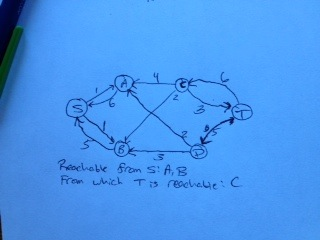
\includegraphics{photo.jpeg} \\(Note the arrow goes from T to D)
\item Bottleneck edges: $(A,C)$, $(B,C)$
\item A three node graph, in a line i.e. $A->B->C$, where the capacity of each edge is 1
\item The bottleneck edges are the edges that connect the verities reachable by $S$ with the vertices from which $T$ is reachable. So we have run the network flow algorithm and are left with the residual graph. On the residual graph, start from $S$ and run explore. Keep track of every vertex visited, because these are reachable by $S$ in the residual graph. For every vertex in this set, get its out edges in the original graph. Now explore these vertices in the residual graph (if they aren't reachable by S, if they are we know that they can't get to T)-- if you can get to $T$ from the new vertex, then awesome, the edge that we went back to the original graph for is a bottleneck edge! This has the potential to take very long, but if we keep track of answers, i.e. from which vertices we can reach $T$ then we shouldn't have visit each vertex and edge more than once, aka linear time.
\end{enumerate}
\newpage
\item
\begin{enumerate}
\item maximize $f_{(s,a)}+f_{(s,b)}$\\
Constraints: $f_{e}\le c_{e}, \forall e\in E$\\
for $u\in \{A,B\}$ $\sum_{(w,u)\in E}f_{wu}=\sum_{(u,w)\in E}f_{uw}$,  flow coming into a vertex equals flow coming out of vertex
\item The dual:
minimize: 
We let $d_{ij}$ be the dual variables corresponding to the capacity upper bounds and let $p_i$ the variable associated with the flow coming into node $i$ equals the flow going out of node $i$.\\
minimize: $c_{sa}d_{sa}+c_{sb}d_{sb}+c_{ab}d_{ab}+c_{at}d_{at}+c_{bt}d_{bt}$\\
Constraints:\\ 
$d_{sa}+p_a-1\ge 0$, $d_{sb}+p_b-1\ge 0$, \\
$d_{ab}-p_a+p_b\ge 0$, $d_{at}-p_a\ge 0$, \\
$d_{bt}-p_b\ge 0$\\
$p_i \ge 0$ for every $i\in V$\\
$d_{ij}\ge 0$ for every $(i,j)\in E$\\
\item 
minimize $\sum_{e\in E}c_{e}y_{e}$\\
Constraints: $y_{ij}-p_i+p_j\ge 0$ for every $(i,j)\in E, i,j\notin \{s,t\}$\\
$y_{si}+x_i\ge 1$\\
$y_{it}-x_i\ge 0$\\
$y_{e}\ge 0$ for every $e\in E$\\
\item We can sum constraints:\\
$\sum_{(i,j)\in E, i,j\notin \{s,t\}}(y_{ij}-x_i+x_j) + \sum_{(s,i)\in E}(y_{si}+x_i) + \sum_{(i,t)\in E}(y_{it}-x_i)\ge 1$\\
$\sum_{e\in E}y_e\ge 1$ \\
because the first term excludes the start and end vertices, and the $+x_i$ in the second term and the $-x_i$ in the third make up for extra values of $x_i$ or $x_j$ in the first term
\item So, for a given cut, $y_e$ represents whether $e$ goes across the cut and $x_u$ represents whether $u$ comes before the cut. For a cut $C=(S,T)$, $y_{ij}=1$ if $i\in S$, $j\in T$, otherwise $y_e=0$, $x_u=1 \forall u\in S$, $x_k=0$ otherwise. This satisfies the constraints in the dual problem and $\sum_{e\in E}c_ey_e$ equals the sum of the capacities of the edges in the cut.
\end{enumerate}
\newpage
\item Soooo lets have $t$ be the number of grams of tomatoes we have,\\
$l$ for lettuce, $s$ for spinach, $c$ for carrot, $o$ for oil.\\
Minimize: $.21t+.16l+3.71s+3.48c+8.84o$\\
Constraints:\\
$.0085t+.0162l+.1278s+.0839c\ge 15$\\
$.0033t+.0020l+.0158s+.0139c+1o\ge 2$\\
$.0033t+.0020l+.0158s+.0139c+1o\le 6$\\
$.0464t+.0237l+.7469s+.8070c\ge 4$\\
$.09t+.08l+.07s+5.082c \le 100$\\
$l+s\le t+c+o$\\
I used: http://www.zweigmedia.com/RealWorld/simplex.html\\
And got:\\
Optimal Solution (all in grams): minimum = 232.5; t = 588.5, l = 584.3, s = 4.163, c = 0, o = 0
\end{enumerate}
\end{document}
